\section{Disturbo d'ansia}

L'ansia è uno stato psichico, prevalentemente cosciente, caratterizzato
da una sensazione di preoccupazione o paura, più o meno intensa o
duratura, che può essere o meno connessa o meno ad uno stimolo specifico
immediatamente individuabile, sia interno che esterno, quindi la si può
considerare come mancata risposta di adattamento dell'organismo ad una
qualsiasi fonte di stress. Così definita, l'\emph{ansia in quanto tale
non ha sempre un significato patologico}, ma è un fenomeno psichico
evolutivamente selezionato per preparare il soggetto ad affrontare le
situazioni stressanti, garantendo così una migliore performance, e ciò
giustifica anche le classiche alterazioni neurovegetative legate
all'ansia, che sono dovute ad un'aumentata attività del simpatico.
L'ansia, inoltre, \emph{non è presente solo nei disturbi d'ansia}, ma la
si può ritrovare, in misura minore o maggiore, in praticamente tutti i
disturbi psichici, per cui \emph{non può essere considerata come un
sintomo patognomonico}.

I \textbf{\emph{disturbi d'ansia}} sono disturbi psichici piuttosto
diffusi nella popolazione generale, tanto che la loro prevalenza
annuale, in pazienti dai 18 ai 54 anni è stimata essere di circa il
13,3\%, quota molto rilevante, basti pensare che i disturbi mentali, nel
loro insieme hanno una prevalenza annuale del 20,9\%. All'interno dei
disturbi d'ansia possiamo poi identificare diverse forme, tra cui le
principali sono le \textbf{fobie} (fobie specifiche e fobia sociale), il
\textbf{disturbo d'ansia generalizzato} (GAD), il \textbf{disturbo di
panico} ed il \textbf{disturbo} \textbf{ossessivo-compulsivo} (DOC).

\subsection{Disturbo di panico e attacco di panico}

Il \textbf{disturbo di panico} è un disturbo mentale relativamente
comune, che affligge fino al 5\% circa della popolazione generale in un
dato periodo della vita, ed è una condizione notevolmente disabilitante,
soprattutto se complicato dall'\emph{agorafobia}, ed anche per il fatto
che si associa spesso comorbilità e determina una notevole riduzione
della qualità della vita. La base eziopatogenetica del disturbo di
panico non è stata ancora compresa in ogni suo aspetto, tuttavia è ormai
certo che vi sia alla base una certa \emph{suscettibilità individuale di
natura genetica}, ed anche alcune \emph{malattie fisiche}, come l'asma,
si associano spesso al disturbo di panico, mentre alcune abitudini di
vita, in particolare il fumo di sigaretta, sembrerebbero in grado di
aumentare il rischio di tale patologia.

È importante, a questo punto, \emph{differenziare l'\textbf{attacco di
panico} dal \textbf{disturbo di panico}}:

\paragraph{L'attacco di panico}

L'ATTACCO DI PANICO secondo il DSM-IV è definito come:

un periodo preciso di intensa paura o disagio, durante il quale 4, o
più, dei seguenti sintomi si sono sviluppati improvvisamente e hanno
raggiunto il picco in 10 minuti:

\begin{itemize}
\item[1.]
  Palpitazioni, tachicardia, cardiopalmo
\item[2.]
  Sudorazione
\item[3.]
  Tremori fini o a grandi scosse
\item[4.]
  Dispnea o sensazione di soffocamento
\item[5.]
  Sensazione di asfissia
\item[6.]
  Dolore o fastidio al petto
\item[7.]
  Nausea o disturbi addominali
\item[8.]
  Sensazioni di sbandamento, di instabilità, di testa leggera o di
  svenimento
\item[9.]
  Derealizzazione (sensazione di irrealtà) o depersonalizzazione: alcuni
  riferiscono che gli sembra di guardare se stessi mentre stanno male o
  che gli sembra di essere collocati fuori dalla realtà.
\item[10.]
  Paura di perdere il controllo o di impazzire
\item[11.]
  Paura di morire
\item[12.]
  Parestesie (sensazioni di torpore o di formicolio)
\item[13.]
  Brividi o vampate di calore
\end{itemize}

Se un pz descrivesse un attacco di panico lo descriverebbe,
generalmente, in questo modo:
\\\\
``Stavo bene, improvvisamente tachicardia, dispnea, la sensazione di
svenire, non riuscivo a spiegare a chi mi ha soccorso cosa stava
succedendo, avevo contrazioni muscolari, paura di morire, è durato più
di mezz'ora''
\\\\
Il pz sta bene e \textbf{improvvisamente} è colpito da qualcosa che gli
determina una repentina e molto intensa attivazione di tutto il sistema
neurovegetativo, soprattutto simpatico. Non è solo quello, perché si
riesce sperimentalmente ad indurre un'attivazione del sistema nervoso
autonomo come quella dell'attacco di panico, in quelli che ne soffrono,
quando stanno bene, con alte dosi di caffeina, o facendo respirare una
miscela d'aria con più anidride carbonica, in questi modi si può indurre
la dispnea con una sensazione molto particolare, cioè che l'aria riesce
a uscire ma fa fatica ad entrare, con una sensazione di morire
soffocati. Tachicardia, palpitazione, dolore retrosternale con
irradiazione al braccio sx (sono molto frequenti in chi ha avuto un
infarto o ha assistito all' infarto di qualcun altro). Brividi che si
alternano a vampate di calore, sudorazione profusa e tremori. Tutto
questo si può indurre, non si può indurre però, o si fa molta più fatica
ad indurre, la componente psichica, che è: paura di morire oppure la
paura che in quel momento si possa perdere il controllo o di impazzire.
\\\\
Arriva improvvisamente tutto questo e dura o pochi minuti o di più, raro
però che superi la mezz'ora.
\\\\
Dopodiché lo lascia in una specie di prostrazione simile al postsbornia
o come se gli fosse passato sopra un rullo compressore.

Così definito, l'attacco di panico può essere di 3 tipi:

\begin{itemize}
\item
  \textbf{\emph{Attacco di Panico Inatteso}}, che compare
  all'improvviso, senza connessioni con l'attività del soggetto o col
  luogo in cui si trova; fulmine a ciel sereno): il pz sta bene e
  l'attacco arriva in qualsiasi momento e in qualsiasi luogo
\item
  \textbf{\emph{Attacco di Panico Situazionale}}, che compare sempre e
  solo quando il paziente si viene a trovare in una determinata
  situazione; \emph{con evitamento fobico:} cioè non avviene dovunque,
  ma solo in determinate situazioni, che però, per poter indurre un
  attacco di panico, devono avere due caratteristiche fondamentali:

  -luoghi da cui può essere difficile andarsene (mezzi di trasporto,
  posti affollati, l'autostrada) ma non perché può succedere un
  incidente, bensì perché il soggetto può sentirsi male e se ne deve
  poter andare da lì

  -luoghi difficilmente raggiungibili dai soccorsi.
\item
  \textbf{\emph{Attacco di Panico Sensibile dalla Situazione}}, che
  compare quando il paziente si trova in una certa situazione, ma non
  sempre.
\end{itemize}

C'è una differenza nelle conseguenze, perché in quello situazionale
basta che il soggetto non vada in quel posto e l'attacco non viene.
Questi pz hanno tutti le loro situazioni che evitano. Negli inaspettati
non si può evitare. Il problema è che sono costantemente in ansia che
gli venga un attacco (ansia anticipatoria). Molti pz hanno anche la
paura delle conseguenze che quest'ansia possa avere sul loro organismo.

\paragraph{Il disturbo di panico}

\emph{\emph{Epidemiologia:}}

Epidemiologicamente, il disturbo di panico ha una prevalenza life-time
stimata dell'\textbf{1,6-2,2\%} nella popolazione generale, ed è \emph{2
volte più comune nelle donne che negli uomini}, esordendo in genere
durante la III decade di vita ed associandosi ad agorafobia nel 30-50\%
dei casi. I parenti di primo grado hanno un rischio 8 volte maggiore nei
familiari di primo grado rispetto alla popolazione generale di
sviluppare un disturbo di panico, il quale spesso può \emph{predisporre
ad altre condizioni psichiatriche}, come l'abuso di alcol e alla
depressione maggiore (la si riscontra nel 50-60\% dei casi di disturbo
di panico, e in 1 caso su 3 lo può precedere).

\emph{\emph{Definizione:}}

IL DISTURBO DI PANICO, secondo i criteri del DSM-V, è una
\emph{condizione patologica che si caratterizza per :}

\begin{itemize}
\item[1.]
  attacchi di panico ricorrenti e inaspettati
\item[2.]
  almeno uno degli attacchi di panico è stato seguito da 1 mese, o più
  di:

\begin{itemize}
\item
  persistente paura che possano comparire altri attacchi o le
  conseguenze degli attacchi
\item
  significativi cambiamenti del comportamento in conseguenza all'attacco
  di panico
\end{itemize}

\item[3.]
  gli attacchi di panico non sono in relazione con abuso di sostanza o
  altre patologie (ipertiroidismo..)
\item
  gli attacchi di panico non sono da confondere con: Disturbo ossessivo
  compulsivo, Disturbo di Fobia sociale, Disturbo post traumatico,
  disturbo di ansia da separazione.
\end{itemize}

\paragraph{Agorafobia}

Strettamente correlata al disturbo di panico è
l'\textbf{\emph{agorafobia}}, definita come una \emph{marcata paura o
ansietà in almeno due condizioni agorafobiche}, come essere fuori di
casa da solo, prendere i trasporti pubblici, stare all'aperto, andare al
cinema, in teatro o nei negozi, o anche stare in fila o in mezzo alla
folla.

Spesso ansia e agorafobia coabitano nello stesso pz. Se il pz va in quel
posto sta male e per evitare di star male (avere un attacco di panico)
in quel posto non ci va.
\\\\
n.b: Attenzione perché esiste un altro disturbo che si chiama fobia
sociale, che è una cosa completamente diversa da questa. Ad esempio la
paura di usare il bagno in presenza di altre persone o la paura di
mangiare e di parlare in pubblico, cioè la paura di far qualcosa per cui
gli altri possono giudicare. La chiamiamo fobia sociale e non ha nulla a
che vedere con l'agorafobia.

Il DSM-IV la definisce come:

\begin{itemize}
\item
  \emph{l'individuo teme e cerca di evitare tutte le situazioni in cui
  la fuga potrebbe essere difficoltosa in caso avesse un attacco di
  panico}
\item
  da ciò deriva che le condizioni agorafobiche suscitano una
  \emph{marcata ansia e paura nel soggetto}, che cerca di evitarle, o al
  più le affronta ma ricercando sempre la presenza di un compagno,
  sebbene sia \emph{consapevole che la sua ansia sia del tutto
  sproporzionata rispetto al pericolo reale legato}.
\item
  La durata dell'agorafobia dev'essere almeno di \textbf{\emph{6 mesi}},
  e deve causare uno stress o un'alterazione significativa nel
  funzionamento sociale e/o occupazionale nel soggetto
\item
  ovviamente il senso di ansia ed intensa paura non devono essere legate
  all'azione fisiologica diretta di sostanze o di condizioni mediche
  generali, e non devono nemmeno essere connessi con un'altra patologia
  psichiatrica.
  \end{itemize}
 
\subsubsection{Terapia del disturbo di panico}

Il trattamento del disturbo di panico si pone come obbiettivi
principali:

\begin{itemize}
\item
  la riduzione della frequenza e dell'intensità degli attacchi di
  panico,
\item
  la riduzione dell'ansia anticipatoria,
\item
  la riduzione dell'evitamento fobico ed il trattamento dell'eventuale
  depressione associata al disturbo di panico.
\end{itemize}

Per questa patologia, quindi, per opzioni terapeutiche sono
essenzialmente due:

\begin{itemize}
\item
  \textbf{Psicofarmaci}, nello specifico antidepressivi ed ansiolitici;
\item
  \textbf{Psicoterapia Cognitivo-Comportamentale}.
\item
  \textbf{Placebo,} il 50\% dei casi è responsivo
\end{itemize}

Questi due approcci terapeutici non si escludono reciprocamente, anzi
\emph{spesso si hanno dei risultati migliori integrandoli assieme}, ed
hanno un'\emph{efficacia che è pressoché sovrapponibile}, anche perché i
disturbi di panico (anzi i disturdi d'ansia in generale) sono le
patologie psichiatriche con la più elevata risposta al placebo.

\paragraph{Psicofarmaci}

Per quanto riguarda gli \textbf{psicofarmaci}, abbiamo due classi
farmacologiche principali più un'altra:

\begin{itemize}
\item
  \emph{\textbf{BENZODIAZEPINE}}

In generale,la maggior parte dei paziente e dei medici generici
preferisce optare per le BENZODIAZEPINE, che danno un effetto immediato,
e spesso il paziente sta molto meglio semplicemente portando con sé il
farmaco, perché si sente ``protetto'' da un eventuale attacco di panico,
anche se \emph{in realtà le benzodiazepine non hanno effetti rilevanti
in acuto}, infatti il diazepam, che è la benzodiazepina con la latenza
più breve, richiede almeno 15 minuti per dare effetti rilevanti, mentre
gli attacchi di panico raramente si estendono per più di 10 minuti, ma
ciò nonostante il farmaco ha dimostrato di possedere comunque un
notevole effetto contro l'ansia anticipatoria (Sono state formulate
anche delle benzodiazepine per via sublinguale, che nonostante abbiano
lo stesso periodo di assorbimento, danno al paziente la sensazione che
l'effetto sia immediato.)
\\\\
Le benzodiazepine sono tra i farmaci in assoluto più soggetti ad abuso,
non solo da parte dei pazienti psichiatrici ma anche da parte di
soggetti che non hanno alcun tipo di patologia psichiatrica
diagnosticata, e dati recenti sembrano dimostrare come questo abuso sia
leggermente più frequente nel sesso femminile rispetto a quello
maschile, tanto che si ritiene che una donna su 5 abbia abusato di
questi composti almeno una volta nella vita, rispetto ad un uomo su 10,
e nonostante la prescrizione delle benzodiazepine si sia ridotta negli
ultimi anni, rimangono comunque tra i farmaci più utilizzati nei centri
di salute mentale.

\emph{\emph{Struttura chimica:}}

Dal punto di vista prettamente chimico, la maggior parte dei composti
usati in ambito clinico sono delle \emph{1,4-benzodiazepine}, e la
maggior parte contiene un gruppo carbammidico nella struttura
eterociclica a 7 atomi; per l'attività sedativo-ipnotica, inoltre, è
importante la presenza di un \emph{sostituente in posizione 7}, nello
specifico un alogeno o un nitrogruppo.

\emph{\emph{Farmacinetica:}}

\begin{figure}[!ht]
\centering
	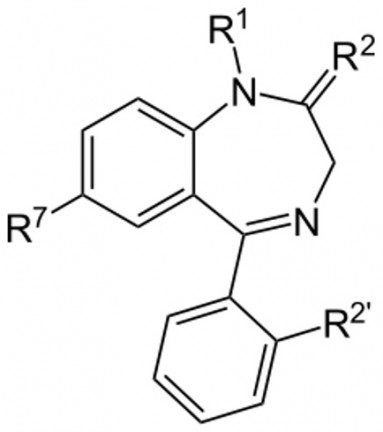
\includegraphics[width=0.3\textwidth]{04/image1.jpeg}
\end{figure}

Dal
punto di vista della \textbf{farmacocinetica}, la \emph{velocità di
assorbimento} orale di questi sedativo-ipnotici dipende da diversi
fattori, in primis dalla loro \emph{liposolubilità}: ad esempio
l'assorbimento del triazolam è molto rapido, essendo questa una molecola
molto liposolubile così come lo è anche il diazepam e del clorazepam, e
la liposolubilità del composto è importante anche nello stabilire la
velocità con cui il farmaco supera la barriera emato-encefalica, andando
ad agire sui suoi bersagli recettoriali, ma è anche importante perché
consente al composto di \emph{superare la barriera emato-placentare},
infatti tutte le benzodiazepine sono controindicate in gravidanze,
poiché potrebbero dare gravi effetti sul feto e sul neonato, con
depressione delle funzioni vitali, e particolare attenzione va anche
posta al \emph{latte materno}, in cui le benzodiazepine si possono
accumulare. Per quanto riguarda il destino metabolico di questi farmaci,
essi vengono \emph{metabolizzati a livello epatico dal sistema del
citocromo P 450}, in particolare il \textbf{CYP3A4}, con processi di
ossidrilazione alifatica ed N-dealchilazione; i metaboliti
successivamente formati vengono quindi coniugati in reazioni di fase II
con l'acido glucuronico, ottenendo composti idrosolubili che vengono
quindi escreti tramite le urine. Tuttavia, molti metaboliti ottenuti
dalle reazioni di fase I sono ancora \emph{farmacologicamente attivi},
per cui l'effetto farmacologico può permanere più a lungo rispetto alla
semplice emivita farmacologica (quindi il loro uso dev'essere
attentamente controllato in caso di insufficienza epatica o epatopatie)
come nel caso del diazepam, che viene convertito in desmetildiazepam e
poi in oxazepam, il quale viene infine coniugato ed escreto con le
urine.

\emph{\emph{Effetti Farmacologici :}}

I principali effetti farmacologici legati alle benzodiazepine sono:

\begin{itemize}
\item
  \textbf{Sedazione ed Effetto Ipnotico};
\item
  \textbf{Effetto Ansiolitico};
\item
  \textbf{Effetto Anticonvulsivante};
\item
  \textbf{Effetto Miorilassante}, con riduzione del tono muscolare,
  sfruttato prevalentemente in ambito anestesiologico.
\end{itemize}

Se si volesse schematizzare, adottando un modello un po' artificioso,
gli effetti principali delle benzodiazepine possono essere così
suddivise:

\begin{itemize}
\item
  L'\emph{effetto ansiolitico} è maggiore con l'\textbf{alprazolam} ed
  il \textbf{lorazepam};
\item
  L'\emph{effetto ipno-inducente} è maggiore con l'\textbf{alprazolam} e
  il \textbf{triazolam};
\item
  L'\emph{effetto anti-convulsivante} è maggiore con \textbf{diazepam}.
\end{itemize}

\emph{\emph{Effetti Indesiderati}}

Un aspetto forse poco noto delle benzodiazepine sono le
\textbf{alterazioni a carico delle funzioni cognitive} causate dall'uso
di questi farmaci: nei pazienti, soprattutto se anziani, il trattamento
con benzodiazepine può dare \emph{alterazioni della capacità di
concentrazione}, un \emph{incremento dei tempi di reazione} ed anche
\emph{fenomeni anmesici}. Tutti questi effetti indesiderati non sono
unici del soggetto anziano, ma possono anche manifestarsi in soggetti
più giovani, anche se spesso in modo meno accentuato.

Le BDZ, in caso di sovraddosaggio, possono causare un \emph{sonno
prolungato} ma senza una depressione seria della funzione respiratoria o
cardiovascolare, tuttavia in pazienti con importanti patologie organiche
come le \textbf{BPCO} o in generale un'\textbf{insufficienza
respiratoria} potrebbero dare una \emph{grave depressione del centro del
respiro, con esiti potenzialmente anche letali}, e per tale motivo la
loro somministrazione è altamente controindicata in questo tipo di
pazienti, così come lo sono in pazienti a cui è stata diagnosticata una
concomitante \textbf{patologia neurologica}, poiché l'assunzione di
benzodiazepine potrebbe in questo caso determinare la comparsa di
\emph{atassia} ed \emph{ipotonia muscolare}.
\\\\
Altri effetti collaterali meno frequenti sono poi le \emph{lipotimie} e
le \emph{disfunzioni sessuali}.
\\\\
Dal punto di vista delle funzioni mentali, come già accennato le
benzodiazepine possono \emph{inficiare la memoria}, più nello specifico
interferiscono coi processi di consolidamento della \emph{memoria
verbale} (tipicamente il paziente riferisce di non riuscire a ricordare
i nomi delle cose o delle persone), e può essere interessata anche la
\emph{memoria a breve termine}, mentre quella a lungo termine è in
genere risparmiata. Si tratta generalmente di un'\textbf{\emph{amnesia
anterograda}}, cioè in questi pazienti si conserva la capacità di
ricordare nozioni o eventi del passato, ma non si riesce a fissare nuove
informazioni, e solo a dosi piuttosto elevate del farmaco può
effettivamente comparire un'amnesia totale, sebbene transitoria.

Da questi dati deriva ovviamente che le benzodiazepine
\emph{nell'anziano sono farmaci da usare con estrema cautela e solo se
necessario}, poiché in questo gruppo di pazienti i processi cognitivi
sono già di per sé compromessi e rallentati, e l'assunzione del farmaco
porterebbe inevitabilmente ad un peggioramento della situazione, dando
anche dei casi di \textbf{pseudo-demenza}. Sempre negli anziani,
inoltre, le benzodiazepine sembrerebbero in grado di suscitare una
particolare \emph{disinibizione comportamentale}, la quale è stata
descritta anche in soggetti affetti da disturbi della personalità, anche
se in quest'ultimo caso manchino ancora dei dati certi.

\emph{\emph{Meccanismo d'Azione:}}

Le benzodiazepine \emph{agiscono legandosi a specifici siti regolatori
allosterici posti a livello del recettore-canale}
\textbf{GABA\textsubscript{A}}, facilitandone l'apertura e
\emph{potenziando quindi l'effetto inibitorio del GABA stesso}. Si deve
tuttavia precisare che, a livello delle diverse aree cerebrali, esistono
diverse isoforme del canale GABA\textsubscript{A}, le quali differiscono
per l'affinità verso le benzodiazepine e quindi nella risposta al
farmaco stesso: le azioni di questi composti si esplicano pertanto in
prevalenza della \emph{corteccia frontale del sistema limbico}, mentre
l'azione anti-convulsivante si svolge a livello del \emph{tronco
encefalico}, gli effetti ipnotici sulla \emph{sostanza reticolare} e gli
effetti amnesici sempre sul \emph{lobo limbico}, in particolare
sull'\emph{ippocampo}.

\emph{\emph{Criteri di Scelta del Farmaco:}}

Uno dei criteri di scelta fondamentale che deve essere sempre preso in
considerazione nel momento in cui si valuta l'uso di una benzodiazepina
è l'\textbf{emivita} del composto stesso, che varia notevolmente da
farmaco a farmaco e consente di distinguere le benzodiazepine in:

\begin{itemize}
\item
  \textbf{\emph{BDZ a lunga emivita}}; come il \emph{diazepam} (Valium),
  che ha un'emivita di 20-100 ore (in alcuni casi arriva anche a 200
  ore!);
\item
  \textbf{\emph{BDZ ad emivita intermedia}}; come il \emph{clonazepam}
  (Rivotril), che ha un'emivita di 18-50 ore;
\item
  \textbf{\emph{BDZ ad emivita breve}}; quali il \emph{lorazepam}
  (Tavor, emivita di 11-20 ore), l'\emph{oxazepam} (Serax, Serenid,
  Serepax, emivita di 8-15 ore) e il \emph{lormetazepam} (Noctamid,
  emivita di 10-12 ore);
\item
  \textbf{\emph{BDZ ad emivita ultrabreve}}, come l'\emph{alprazolam}
  (Xanax, emivita di 6-12 ore) e il \emph{triazolam} (Halcion, emivita
  di 2-5 ore).
\end{itemize}

Le diverse emivite di questi composti dipendono essenzialmente dalla
loro \textbf{velocità di eliminazione}, infatti le benzodiazepine
differiscono notevolmente tra loro nella velocità con cui sono
metabolizzate a livello epatico e poi eliminate dall'organismo tramite
le urine: ad esempio l'emivita del triazolam (Halcion) è solo di 2-5
ore, mentre quella del diazepam (Valium) è molto maggiore, anche di 100
ore o più, e questo perché a livello epatico il diazepam viene
convertito in \emph{desmetildiazepam}, che conserva un'azione
farmacologica notevole, diversamente da quanto avviene col triazolam,
che non dà origine in maniera significativa a composti attivi dopo la
sua metabolizzazione. Chiaramente, se da un lato la lunga emivita
garantisce una copertura maggiore dei sintomi, dall'altro, a seguito di
un'assunzione giornaliera protratta, il farmaco \emph{può accumularsi
nei diversi tessuti}, in particolare nel \emph{tessuto adiposo}, per cui
la rimozione dell'effetto farmacologico avviene molto più lentamente.
\\\\
Per questi motivi, in un soggetto depresso ma senza problematiche
particolarmente gravi è preferibile somministrare una BDZ a breve
emivita, che garantisca un buon effetto ipnotico alla sera ma che non
dia disturbi cognitivi al mattino seguente, come ad esempio il
lormetazepam (Minias), ma se il paziente ha un'insonnia di tipo
intermedio o terminale, con frequenti risvegli notturni, allora è bene
dare un farmaco ad emivita media, come l'alprazolam (Xanax), mentre le
benzodiazepine a lunga emivita, come il diazepam (Valium) sono oggi
molto meno usate che in passato, tanto che si preferisce non usarle
nemmeno in pazienti con funzionalità epatica integra, a meno che non sia
necessario un effetto terapeutico molto prolungato o, per motivi di
compliance, non sia possibile fare più somministrazioni giornaliere.
\\\\
Se invece quello che si ricerca è un effetto prevalentemente
\emph{ansiolitico}, è bene ricorrere ad una benzodiazepina ad emivita
intermedia, come l'\textbf{alprazolam}, che viene dato prima a dosi
basse, aumentando poi la dose sino a portarla a regime, così da evitare
gli effetti collaterali connessi col suo utilizzo.
\\\\
Recentemente, peraltro, sono stati introdotti in clinica anche alcuni
nuovi \emph{farmaci melatonino-simili}, come l'\textbf{agomelatina}
(Valdoxan/Thymanax), che ha una struttura simile a quella della
melatonina, ed agisce da agonista nei confronti dei recettori MT1 e MT2,
per cui possiede una blanda attività antidepressiva ed è anche utile per
regolarizzare il ciclo sonno-veglia, per cui se possibile si dovrebbe
cercare di sfruttare questi nuovi composti piuttosto che ricorrere con
eccessiva frequenza alle benzodiazepine.

\emph{\emph{Tolleranza e Dipendenza:}}

Uno dei principali problemi connessi con l'uso delle benzodiazepine è
che, se la loro somministrazione viene protratta nel tempo, si sviluppa
frequentemente un meccanismo di \textbf{tolleranza}, che è legata sia ad
un aumento del metabolismo dei farmaci a livello epatico, sia ad alcune
modificazioni recettoriali a livello delle membrane sinaitiche, tali da
richiedere un aumento progressivo delle dosi per raggiungere lo stesso
effetto che si otteneva prima con una dose minore. Strettamente
correlata col fenomeno della tolleranza è poi la \textbf{dipendenza}
dalla benzodiazepine, che è \emph{più comune in soggetti con disturbi
della personalità o in soggetti che hanno già una storia pregressa di
abuso d'alcol o sostanze}. Le benzodiazepine possono infatti dare sia
una \textbf{\emph{dipendenza fisica}} che una \textbf{\emph{dipendenza
psicologica}}: nella dipendenza psicologica tutte le attività svolte dal
soggetto diventano subordinate all'uso o all'acquisizione della sostanza
nei confronti della quale si ha la dipendenza, per cui il farmaco
diventa le preoccupazione principale della giornata del soggetto, mentre
nella dipendenza fisica compare una vera e propria sindrome da astinenza
legata alla mancata assunzione del farmaco, e in questi casi la
dipendenza da BDZ può creare non pochi problemi di diagnosi
differenziale, in quanto si manifesta con una sintomatologia in gran
parte sovrapponibile ai disturbi di panico.

Di fronte a questi problemi, nel caso in cui si ritenga opportuna la
sospensione del trattamento farmacologico è importante che il dosaggio
delle benzodiazepine sia \emph{ridotto in maniera graduale}, e
dev'esserci un impegno congiunto nell'affrontare degli incontri
medico-paziente più frequenti, ricordando al paziente il ruolo delle
benzodiazepine e le problematiche connesse alla loro assunzione prima di
intraprendere la terapia stessa.

\begin{figure}[!ht]
\centering
	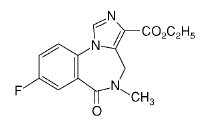
\includegraphics[width=0.5\textwidth]{04/image2.jpeg}
\end{figure}

In
caso di \textbf{intossicazione}, infine, questa potrebbe risultare molto
seria in soggetti che hanno una pregressa patologia polmonare o
cardiocircolatoria di base, in quanto si potrebbe instaurare una
\emph{depressione del centro del respiro o di altri centri del tronco
encefalico}, e in questi casi è necessario intervenire con il
\textbf{\emph{flumazenil}}, un antagonista competitivo delle
benzodiazepine, che si lega al sito specifico di questi farmaci sul
recettore GABA\textsubscript{A} ma senza facilitarne l'apertura.


\item
  \textbf{\emph{ANTIDEPRESSIVI:}}

Gli ANTIDEPRESSIVI presentano il vantaggio di \emph{non causare
sedazione}, \emph{né assuefazione o dipendenza}, ma hanno il limite di
avere un \emph{periodo di latenza elevato} (occorrono almeno 2-3
settimane perché l'effetto farmacologico diventi chiaramente manifesto)
e paradossalmente possono causare dei \emph{sintomi panic-like} (perché
molti bloccano la ricaptazione della noradrenalina, per cui promuovono
un'attivazione del sistema nervoso simpatico), mentre le benzodiazepine
hanno il vantaggio di dare una \emph{rapida comparsa dei loro effetti},
ma d'altro canto \emph{causano sedazione, assuefazione e dipendenza}.

GlI \emph{\textbf{SSRI}} sono sempre da preferire ai TCA per i minori
effetti collaterali: questi farmaci hanno infatti \emph{minori effetti
anti-colinergici e cardiovascolari}, \emph{non provocano sedazione o
aumento ponderale}, sebbene possano comunque acere \emph{effetti sulla
sfera sessuale}, \emph{nausea, cefalea o insonnia}, così come gli
\emph{spiacevoli sintomi ``panic-like''} legati all'attivazione del
simpatico. A ciò va poi aggiunto che gli SSRI hanno una \emph{potenza
maggiore rispetto ai TCA}, per cui consentono al paziente di assumere un
numero minore di compresse, spesso permettendo anche una
mono-somministrazione giornaliera del farmaco. Gli SSRI attualmente in
commercio sono 6 (citalopram, escitalopram, paroxetina, sertralina,
fluoxamina e fluvoxetina) e sono tutti caratterizzati dall'agire tramite
un \textbf{blocco del trasportatore della serotonina} presente a livello
sinaptico, mentre differiscono leggermente tra loro per le ulteriori
azioni farmacologiche (vedi tabella).

\begin{table}
%\caption{Please write your table caption here}
\begin{tabular}{p{0.3\textwidth}p{0.3\textwidth}p{0.3\textwidth}}
\hline\noalign{\smallskip}
\textbf{\emph{Farmaco}} & \textbf{\emph{Bersaglio d'Azione Primario}} & \textbf{\emph{Altri Effetti}}  \\
\noalign{\smallskip}\svhline\noalign{\smallskip}

Escitalopram & SERT (Trasportatore della SERotonina) & - \\
Citalopram & SERT & Blocco recettori H1 \\
Sertralina & SERT & Blocco DAT, interazione coi recettori $\sigma$ degli oppioidi \\
Fluvoxamina & SERT & Interagisce coi CYP3A4 e CYP1A2, interazione coi recettori $\sigma$ degli oppioidi \\
Fluoxetina & SERT & Blocco NET, Blocco recettori 5-HT\textsubscript{2}, interagisce col CYP3A4 e CYP2D6 \\
Paroxetina & SERT & Interagisce col CYP2D6, blocco dei recettori M1, blocco del NET, interagisce con NOS \\

\noalign{\smallskip}\hline\noalign{\smallskip}
\end{tabular}
\end{table}


Visto che gli antidepressivi, sia gli SSRI che i TCA, necessitano di
\emph{almeno 2 settimane per dare i loro effetti}, \emph{in genere li si
associa alle benzodiazepine}, in modo da non lasciare ``scoperto'' il
paziente, poi l'ansiolitico può essere gradualmente tolto, in quanto gli
antidepressivi raggiungono il picco della loro azione in circa 8-12
settimane, e vanno mantenuti per almeno 6 mesi dopo la risposta
iniziale.

\item
  \textbf{\emph{BETA BLOCCANTI:}}

Altri farmaci spesso somministrati ai pazienti ansiosi sono i
\textbf{$\beta$-bloccanti} in monoterapia, i quali non si sono però dimostrati
efficaci nel ridurre la frequenza degli attacchi di panico o i sintomi
fobici, sebbene siano utili per il trattamento della sintomatologia
neurovegetativa.
\end{itemize}

\paragraph{Psicoterapia cognitivo-comportamentale}

Per quanto riguarda invece la \textbf{\emph{psicoterapia cognitivo-comportamentale}}, essa prevede:

\begin{itemize}
\item
  una \emph{prima fase di psicoeducazione}, in cui si cerca di informare
  il paziente e di fargli comprendere la propria patologia,
\item
  poi si deve puntare sul \emph{monitoraggio costante dei sintomi in
  relazioni agli stimoli causali}, così da contrastare l'insorgenza
  dell'attacco di panico, e questo può essere ottenuto mediante
  l'apprendimento di specifiche \emph{tecniche di respirazione} ed una
  \emph{ristrutturazione cognitiva}, che consente al paziente di
  controllare il timore delle conseguenze dei sintomi, in modo da
  consentirgli di vincere l'ansia anticipatoria e riuscire così ad
  affrontare le situazioni temute.
\end{itemize}

\paragraph{Decorso}

Per quanto riguarda il decorso del disturbo di panico, vari studi hanno
evidenziato che, dopo 4-6 anni dal trattamento, il 30\% dei pazienti si
trova in una condizione di benessere, il 40-50\% sta meglio ma conserva
un certo grado di sintomatologia, e solo il 20-30\% non mostra alcun
miglioramento o addirittura è peggiorato, mentre negli studi a lungo
periodo (20 anni), il 50\% dei pazienti si mantiene senza attacchi, il
30\% ha ancora sintomi, ma senza agorafobia o depressione, mentre il
10\%, pur essendo senza attacchi rilevanti, soffre di depressione o ha
comunque un certo grado di compromissione sociale. Tali dati sono molto
significativi, anche perché i pazienti con disturbo di panico tendono a
ricorrere al PS o all'intervento medico molto più frequentemente
rispetto alla popolazione generale, basti pensare che i pazienti ansiosi
sono responsabili del 6-12\% di tutte le visite ambulatoriali, si
rivolgono al PS circa 10 volte più spesso rispetto ai soggetti non
ansiosi e nel 70\% dei casi vengono valutati da almeno 10 medici prima
di giungere alla diagnosi corretta. Tipici sintomi somatici connessi col
disturbo di panico sono il \textbf{dolore toracico} e le
\textbf{palpitazioni}, per cui la diagnosi differenziale, che spesso
preoccupa notevolmente il paziente stesso, riguarda le patologie
cardio-vascolari: il dolore toracico dell'attacco di panico, tuttavia, è
un \emph{dolore atipico}, cioè \emph{non è retrosternale}, \emph{non è
legato a sforzo} e \emph{non passa col riposo o con la nitroglicerina},
come invece avviene nell'angina pectoris, per cui se il dolore è
atipico, il paziente è relativamente giovane, di sesso femminile, non ha
storia pregressa di coronaropatia ed ha anche elevati punteggi ai test
per l'ansia, la diagnosi di disturbo di panico è molto probabile, ed
anche le palpitazioni sono piuttosto comuni in questi paziente, tanto
che le cause psichiatriche sono al secondo posto, dopo quelle cardiache,
per lo sviluppo del cardiopalmo. Bisogna infine aggiungere, per
completezza, che alcuni studi avrebbero individuato una maggior
incidenza di \textbf{prolasso della valvola mitrale} in soggetto con
disturbo di panico, la il nesso causale tra queste due forme patologiche
non è stato ancora ben compreso.

\subsection{Disturbo ossessivo-compulsivo}

Caso clinico: \emph{ragazza 22-23 anni si reca a fare la babysitter e la
famiglia le affida un bambino di circa un anno e mezzo. Mentre sta
tenendo il bambino sente alla radio degli aggiornamenti sul caso del
delitto di Cogne: alla radio riferiscono che la madre era accusata di
aver ucciso il bambino in un raptus di follia. La ragazza ha il dubbio
di poter avere anche lei un raptus e lanciare giù dalla finestra il
bambino che le è stato affidato. Per la paura mette in atto tutta una
serie di provvedimenti atti ad impedirle di far male al bambino: abbassa
tutte le tapparelle, chiude il bambino a chiave in una stanza e nasconde
la chiave, prova a sentire il suo medico per sentire se fosse in grado
anche lei di fare come la Franzoni. Il medico, però, è a fare le visite
domiciliari e perciò la ragazza terrorizzata, in attesa di poter
ricontattare il medico si lega alla sedia con tutto ciò che riesce a
trovare; lascia libero solo un braccio in modo da poter usare il
telefono.}

\emph{Qual era il rischio per questo bambino di essere lanciato dalla
finestra?}

\emph{Esiste davvero il raptus?}

\emph{Il raptus non esiste, questo è dimostrato dal fatto che la
Franzoni non ha avuto un episodio di raptus (evolutosi in pochi
secondi), ma già ore prima aveva contattato la guardia medica in stato
ansioso dicendo che il suo bambino stava male.}

\emph{Questa situazione è molto diversa da quelle mamme estremamente
impulsive che perdono il controllo e sono talmente arrabbiate ed
esasperate che fanno del male al bambino. Non è un raptus, ma è
un'impulsività che non riesce più a essere frenata.}

\emph{La babysitter in realtà non era pericolosa, pur avendo un problema
di aggressività: l'idea di provare anche un minimo di rabbia è così
pericoloso da non poter nemmeno essere pensato, in quanto per questi
pazienti ciò che viene pensato automaticamente si realizza.}

Il DISTURBO OSSESSIVO COMPULSIVO è un disturbo di ansia che si
caratterizza per la \emph{presenza contemporanea di \textbf{ossessioni}
e di \textbf{compulsioni}}, che causano al paziente una notevole perdita
di tempo (in genere più di un'ora al giorno) o causano un
malfunzionamento sociale o occupazionale rilevante al paziente.

\paragraph{Ossessioni}

Secondo i criteri del DSM, l'\textbf{ossessione} viene definita come:
una \emph{condizione caratterizzata dalla presenza di pensieri (}possono
essere di qualsiasi tipo, ma quelle che angosciano di più il paziente
sono quelle con risvolti aggressivi) \emph{o bisogni ricorrenti o
persistenti} che, ad un certo punto durante il disturbo, vengono
\emph{sperimentati dal paziente come intrusivi, indesiderati e/o
disturbanti}, tanto da causare \emph{ansia} o \emph{paura} nel paziente,
il quale \emph{tenta di sopprimerli o di ignorarli}, oppure cerca di
\emph{neutralizzarli ricorrendo ad altri pensieri o azioni}.
\\\\
L'idea ossessiva, si distingue quindi dall'idea prevalente per il fatto
di essere \emph{egodistonica}, mentre l'altra è ego sintonica, \emph{non
ha rapporti diretti con l'affettività}, \emph{non viene accettata dal
paziente} (\textbf{fenomeno dello ``psichismo di difesa''}), viene
\emph{criticata come assurda} e \emph{limita l'espressione della
personalità} (al contrario l'idea prevalente può essere connessa ad
attività creative).
\\\\
L'ossessione, inoltre, può essere facilmente distinta dal delirio per la
presenza della cosiddetta ``\textbf{meità}'', cioè ``\emph{l'io penso}''
Il paziente riferisce di fare l'azione in prima persona, quindi non è
posseduto da un'altra entità, nonostante l'azione non sia propria del
paziente.

Nei paziente deliranti la meità viene persa, poiché nel delirio si ha
certezza delle proprie credenze. Quindi è diverso dalle
\textbf{esperienze di passività} tipiche delle psicosi, dove tutto è
vissuto come se fossi un contenitore, un burattino e io facessi e
pensassi cose imposte da altri; si vive come posseduti da altri.

\emph{\emph{CASI CLINICI:}}

\begin{itemize}
\item
  \emph{Arriva una suora in ambulatorio che afferma di essere impazzita
  perché nella testa continua a bestemmiare. Cerca di fermarsi ma non
  riesce a bloccare questi pensieri. Questa situazione è diversa
  dall'esperienza di passività (esempio delirio di possessione
  demoniaca), perché il pensiero è riconosciuto come il proprio pur
  essendo egodistonico.}
\item
  \emph{Paziente si presenta in ambulatorio raccontando che gli si
  presentano nella mente delle immagini insistenti di presentatori TV
  che dicono porcate e che non riesce a eliminare. Le immagini sono
  proprie ma vissute come assurde rispetto al proprio carattere.}
\item
  \emph{Madre sente un fatto di cronaca dove una madre ha accoltellato i
  propri figli e le sorge il dubbio insistente di poter compiere lo
  stesso crimine. Per evitare di accoltellarli nasconde i coltelli e
  tutti gli oggetti appuntiti e, inoltre, fa un tentativo notturno
  entrando in camera dei figli con un coltello per vedere se provasse il
  desiderio di accoltellarli. Nonostante i vari tentativi si è convinta
  di poterlo fare e per questo motivo ha mandato i figli dalla madre e
  per poterli vedere bisognava che ci fosse presente qualcuno per
  controllarla.}
\item
  \emph{Uomo che si presenta dicendo che ha rovinato la famiglia perché
  è diventato omosessuale. Ciò è dovuto al fatto che ha sognato di
  andare in moto stretto ad un suo collega e nel sogno gli era piaciuto.
  Per verificare di essere realmente omosessuale aveva comprato riviste
  omosessuali, ma gli facevano schifo. Nonostante questo, non si era
  convinto e faceva anche delle prove entrando di soprassalto
  nell'ufficio del collega per verificare che non provasse sensazioni
  strane.}
\item
  \emph{Paziente si presenta in ambulatorio essendo convinto di aver
  contratto l'HIV dopo rapporti non protetti perché gli era venuto un
  mal di gola, nonostante le analisi del sangue fossero negative. Dopo
  un anno e mezzo richiama dicendo che gli è venuto il dubbio di potersi
  buttare giù dalla finestra e per questo motivo passa a circa due metri
  dalle finestre. Infine dopo circa due anni richiama richiedendo un
  certificato dove si afferma che non è omosessuale perché ha avuto
  delle prestazioni sessuali scadenti con la nuova morosa e qualche
  giorno prima i suoi amici l'hanno chiamato ``culattone'' e perciò gli
  è davvero venuto il dubbio di esserlo.}
\item
  \emph{Paziente si presenta in ambulatorio essendo convinta di avere la
  leucemia perché lavandosi i denti le erano sanguinate le gengive.
  Nonostante avesse fatto le analisi del sangue e queste fossero
  risultate negative, era convinta che fossero sbagliate e chiedeva ai
  medici se esisteva una leucemia con emocromo normale.}
\item
  \emph{Paziente si era convinta di ``fare la stupida'' con i passanti e
  che fosse rimasta incinta con questi ipotetici rapporti nonostante
  fosse in menopausa e l'ecografia fosse negativa.}
\item
  \emph{Paziente dopo aver ascoltato un programma televisivo in cui
  parlavano di melanoma e dei metodi per riconoscerlo, si era convinto
  di avere un melanoma in quanto presentava un nevo irregolare. Il
  paziente si era subito presentato in pronto soccorso la notte stessa
  per essere visto in urgenza ma, poiché i medici al triage gli avevano
  spiegato che la dermatologia non era aperta per questo tipo di
  patologie nelle ore notturne, si era arrabbiato temendo che in poche
  ore il tumore avrebbe potuto ucciderlo. }
\end{itemize}

\paragraph{Compulsioni}

La \textbf{compulsione}, invece, viene definita come una
\emph{condizione che si caratterizza per la presenza di comportamenti o
atti mentali ripetitivi}, che il soggetto sente \emph{guidati dalla
necessità di rispondere ad un'ossessione} o ad una regola che dev'essere
applicata in maniera molto rigida.
\\\\
Questi comportamenti o atti mentali sono finalizzati al \emph{prevenire
o al ridurre l'ansia e lo stress}, o per \emph{impedire qualche evento o
situazione temuta}, sebbene essi non siano in realtà connessi
realisticamente con ciò che il paziente suppone vadano a prevenire,
oppure sono chiaramente eccessivi.
\\\\
Il soggetto li riconosce come eccessivi o irragionevoli, ma, nonostante
questo, non riesce a esimersi dall'eseguire queste azioni.

\emph{\emph{CASI CLINICI:}}

\begin{itemize}
\item
  \emph{Ragazzo si presenta in ambulatorio con il padre e sulla porta
  dello studio prima di entrare cammina avanti e indietro per circa 5
  minuti. Qualche giorno prima il ragazzo, litigando con un suo amico,
  gli aveva tirato un accidente e, per evitare che questo si avverasse
  davvero, si sentiva costretto a compiere questa azione un certo numero
  di volte.}
\item
  \emph{Paziente che, prima che tutta la famiglia potesse andare a
  letto, li faceva lavare con l'alcol: il marito, se non si lavava,
  doveva dormire sul divano. Inoltre era capitato che la madre al
  supermercato avesse incontrato un suo amico tossicodipendente e quindi
  la paziente l'aveva obbligata a buttare via la spesa appena fatta,
  perché credeva che fosse stata contaminata.}
\item
  \emph{Paziente che tutte le volte che esce nel cortile di casa deve
  farsi la doccia.}
\item
  \emph{Paziente che faceva il rappresentante di generi alimentari e a
  fine giornata doveva fare il riepilogo delle vendite davanti ai
  genitori più volte e se i genitori si rifiutavano si buttava a terra
  disperato.}
\item
  \emph{Paziente che aveva avuto dei contrasti con il comune e che per
  camminare sul suolo del comune aveva delle scarpe apposite che dopo
  buttava via. Una sera, a cena con la figlia, questa gli raccontò di
  essere stata in comune e lui allora, subito preoccupato, le chiese che
  scarpe aveva usato e gliele buttò nel camino.}
\item
  \emph{Paziente che mentre stava guidando sentiva un rumore provenire
  dalle ruote ed era convinto di avere investito qualcuno. Ad un
  incrocio aveva visto un ciclista passare e poi dopo non l'aveva più
  rivisto, finché il giorno dopo aveva letto sul giornale che un
  ciclista era stato investito. Si era convinto quindi che si trattasse
  proprio del ciclista che aveva visto e che fosse stato lui stesso ad
  investirlo. Era andato in ospedale a scusarsi con il ciclista, il
  quale ovviamente aveva smentito questa sua convinzione. }
\item
  \emph{Paziente dopo aver portato a scuola il figlio è stato preso da
  un incontrollabile bisogno di masturbarsi. Entra quindi nei bagni
  della scuola e si masturba, ma, arrivato a casa, si convince che ci
  fossero delle telecamere che l'hanno ripreso e che quindi era
  spacciato: le forze dell'ordine, vedendo il video, avrebbero
  certamente pensato che lui fosse un pedofilo e quindi sarebbero venuti
  ad arrestarlo. E anche se dopo qualche giorno non erano venuti ad
  arrestarlo, viveva nell'angoscia. }
\end{itemize}

Ovviamente, le ossessioni e le compulsioni non devono essere dovute
all'effetto fisiologico diretto di una sostanza o di una condizione
medica generale, ed il contenuto di queste manifestazioni non è
ristretto ai sintomi di altri disturbi mentali.
\\\\
Il DSM, inoltre, raccomanda di specificare se il DOC è associato ad una
\textbf{buona capacità di insight}, cioè se il paziente si rende conto
che le sue credenze sono false o probabilmente false, o se vi è una
\textbf{scarsa} o \textbf{del tutto assente capacità di insight}.
\\\\
Il DOC è quindi una patologia psichiatrica complessa, classificato tra i
disturbo d'ansia perché questa è la sua componente centrale, sebbene il
ruolo dell'ansia nella formazione dei sintomi è ben lontana dall'essere
chiarita. Caratteristica peculiare del DOC è la \textbf{\emph{fusione di
pensiero ed azione}}: i pazienti con DOC credono che pensare un evento
negativo lo possa far accadere, e che quindi pensare ad un evento
catastrofico equivalga eticamente a compierlo. Tipiche del DOC sono
anche varie \emph{alterazioni dell'attenzione e della vigilanza}, che
risultano aumentate per quelle parole che hanno un contenuto di
``contaminazione'', cioè ricordano maggiormente le parole a contenuto
negativo e vengono dimenticate più difficilmente. Frequente è anche
l'\emph{incapacità di inibire o spostare l'attenzione da pensieri o
azioni che creano disagio ad altri più piacevoli}, spesso assieme anche
ad alterazioni delle strategie organizzative e rallentamento
psicomotorio, che è conseguente al deficit delle strategie esecutive e
dell'attenzione e al dubbio sulle decisioni.
\\\\
Il disturbo ossessivo-compulsivo ha una \emph{prevalenza life-time}
stimata del \textbf{2-3\%}, e presenta un'età media di esordio attorno
ai \emph{20 anni}, con una leggera predilezione per il \emph{sesso
femminile}.
\\\\
All'interno del DOC si possono poi distinguere diversi sottotipi, come:

\begin{itemize}
\item
  il \textbf{DOC di contaminazione/lavaggio},
\item
  il \textbf{DOC di controllo},
\item
  quello di \textbf{collezione}
\item
  quello di \textbf{simmetria/ordine}.
\end{itemize}

Il decorso di questo disturbo è tendenzialmente cronico con fluttuazioni
di intensità dei sintomi, alcuni dei quali possono persistere anche dopo
un trattamento efficace, e spesso vi è un notevole intervallo di tempo
tra l'esordio dei sintomi e la diagnosi del DOC (in media 9 anni!).
\\\\
L'eziopatogenesi del DOC non è stato ancora ben chiarito, tuttavia è
ormai ampiamente accettato che questo disturbo ha una \emph{base
genetica}, come dimostrato dal fatto che i familiari di primo grado di
un paziente con DOC hanno un rischio maggiore di sviluppare un disturbo
analogo, mentre tra gemelli omozigoti vi è un 67\% di concordanza,
rispetto al 31\% tra gemelli dizigoti, e vari studi hanno ipotizzato un
ruolo dei polimorfismi dei geni che codificano per il
\emph{trasportatore ed i recettori della serotonina}, nonché per i
\emph{recettori D4} della dopamina.
\\\\
Altri studi hanno poi messo in luce diverse alterazioni
neuro-funzionali: nell'animale, infatti, l'attivazione della corteccia
pre-frontale e del nucleo caudato si associa a comportamenti ripetitivi
indotti da agonisti dopaminergici, mentre nell'uomo lesioni traumatiche
della corteccia orbito-frontale determina la comparsa del DOC, anche in
assenza di pregressi sintomi ossessivo-compulsivi, i quali possono
comparire anche in patologie in cui si ha una compromissione dei gangli
della base, come le PANDAS, e la terapia contro il DOC è in grado di
modificare positivamente l'attività pre-frontale e sottocorticale.
\\\\
Queste evidenze hanno portato alla formulazione di \emph{due ipotesi
principali} per giustificare lo sviluppo del DOC, cioè l'\textbf{ipotesi
serotoninergica} e l'\textbf{ipotesi dopaminergica}: nella prima è
supportata dal miglioramento dei sintomi con la somministrazione di
SSRI, mentre la somministrazione di mCPP, un agonista serotoninergico
peggiora i sintomi; la seconda ipotesi si basa invece sull'osservazione
che l'amfetamina induce movimenti ripetitivi, mentre la cocaina accentua
i tic, e l'iperattività dopaminergica potrebbe essere secondaria alla
disfunzione del sistema serotoninergico.

\subsubsection{Disturbi dello spettro ossessivo}

Strettamente connessi col DOC sono i cosiddetti \textbf{\emph{Disturbi
dello Spettro Ossessivo}}, come la \emph{dismorfofobia},
l'\emph{ipocondria} e la \emph{sindrome di Tourette}, che spesso si
associano al DOC propriamente detto, ma non bisogna dimenticare anche il
\emph{disturbo del controllo degli impulsi} (cleptomania,
tricotillomania, gioco d'azzardo, autolesionismo e comportamenti
sessuali compulsivi), l'\emph{anoressia nervosa restrittiva} e le
\emph{coree di Sydenham e di Hungtington}.
\\\\
Forma peculiari di DOC sono poi le \textbf{\emph{PANDAS}} (Pediatric
Autoimmune Neuropsychiatric Disorders Associated with Streptococcal
Infection), condizioni che si caratterizzano per la \emph{presenza di
sintomi ossessivi-compulsivi ed anomalie neurologiche}, come tic,
iperattività, movimenti coreiformi e deficit cognitivi. Possono poi
essere presenti anche labilità emotiva, ansia, irritabilità, incubi
notturni e comportamenti oppositivi. L'esordio delle PANDAS è in genere
in \emph{età pre-puberale} (in media attorno ai 6-7 anni), è
\emph{improvviso ed esplosivo}, con un decorso caratterizzato da
esacerbazioni e remissioni. La diagnosi è relativamente semplice, vista
le relazione temporale tra la comparsa dei sintomi, le esacerbazioni e
l'\textbf{infezione streptococcica}, che in genere precede l'esordio di
circa 6 settimane. Dal punto di vista della fisiopatologia, le PANDAS
sembrerebbero dovute appunto ad un'infezione streptococcica che si
sviluppa i pazienti con una certa suscettibilità genetica (in
particolare è stato molto studiato il ruolo dell'antigene D8/17 dei
linfociti B), per cui si viene a creare una \emph{risposta immunitaria
anomala con alterazioni infiammatorie a carico dei \textbf{gangli della
base}}, che danno appunto sintomi neuropsichiatrici. Il trattamento di
questi disturbi adolescenziali e prepuberali si avvale per prima cosa di
una \emph{terapia cognitivo-comportamentale}, e come trattamento di
seconda linea si ricorre alla somministrazione di \emph{antidepressivi
SSRI}, eventualmente associati alla CBT.

\subsubsection{Terapia del DOC}

Per quanto riguarda la \textbf{\emph{terapia}} del disturbo ossessivo
compulsivo, anche in questo caso si hanno diverse opzioni terapeutiche,
quali:

\begin{itemize}
\item[1.]
  la somministrazione di \textbf{psicofarmaci} (in particolare
  \emph{SSRI})
\item[2.]
  la \textbf{psicoterapia} \textbf{cognitivo-comportamentale}
  (\textbf{CBT}),
\item[3.]
  diversamente dal disturbo di panico, nel DOC la risposta al placebo è
  scarsissima.
\end{itemize}

In genere, nelle \emph{forme lievi/moderate} di DOC si ricorre prima
alla \emph{terapia cognitivo-comportamentale}, e solo come seconda linea
si può optare per l'uso di un \emph{SSRI}, eventualmente associato alla
CBT.

Nelle forme più \emph{severe} si parte direttamente con un \emph{SSRI} o
con l'\emph{associazione SSRI con CBT}.

\paragraph{Psicofarmaci}

\emph{\emph{Trattamento:}}

Nel trattamento farmacologico del DOC è fondamentale scegliere con
attenzione il farmaco e determinare la dose efficace, nonché la durata
appropriata del trattamento, inoltre bisogna valutare con cura il
trattamento dei pazienti pediatrici ed adolescenti.
\\\\
Per quanto riguarda il primo punto, cioè la scelta del farmaco, diversi
studi hanno evidenziato che tutti gli \textbf{SSRI} e la
\textbf{cloripramina} (un TCA relativamente selettivo per il sistema
serotoninergico, è più potente rispetto agli SSRI, ma ha anche più
effetti indesiderati rispetto a questi) hanno un'efficacia superiore al
placebo, mentre gli altri antidepressivi non si sono dimostrati
superiore al placebo.
\\\\
La dose standard del farmaco corrisponde in genere alla stessa dose
usata nella fase acuta, e le linee guida raccomandano di \emph{visitare
mensilmente il paziente per i primi 3-6 mesi} dall'inizio del
trattamento acuto, e di \emph{mantenere la terapia farmacologica per
almeno 1-2 anni}, che dev'essere tolta in maniera graduale e può essere
eventualmente da una terapia a lungo termine a scopo profilattico se si
verificano 2-4 riacutizzazioni severe oppure 3-4 riacutizzazioni lievi o
moderate.
\\\\
Bisogna sempre fare attenzione alla sospensione della terapia del DOC,
perché non è infrequente riscontrare un peggioramento dei sintomi nelle
prime 4-8 settimane dalla sospensione degli SSRI, anche dopo un lungo
periodo di trattamento.

\emph{\emph{Risposta al trattamento:}}

Per quanto riguarda la risposta al trattamento, circa il 40-60\% dei
pazienti presenta un miglioramento medio dei sintomi dopo trattamento
con SSRI, ma \emph{raramente si arriva alla remissione completa}, pur
permettendo ai pazienti di lavorare, farsi una famiglia ed una vita
sociale attiva.
\\\\
Sono \textbf{fattori prognostici negativi}, predittivi di una minor
risposta agli SSRI, una \emph{precoce età di esordio}, la \emph{presenza
di notevoli compulsioni}, la \emph{maggior gravità dei sintomi}, il
\emph{decorso cronico}, la presenza di \emph{ADHD} e di \emph{tics},
nonché l'\emph{associazione con disturbi di personalità} (DP
schizotipico).
\\\\
In alcuni casi si può avere una resistenza al trattamento farmacologico,
che talvolta richiede però fino a 6 mesi per manifestarsi pienamente,
per cui le linee guida consigliano un cambiamento di farmaco dopo 8-12
settimane di non risposta o risposta parziale alla dose massima di un
SSRI, e in questi casi si ha una probabilità del 40\% di avere una
risposta ad un secondo SSRI. Se nonostante ciò si ha un fallimento con
2-3 SSRI, è bene passare alla psicoterapia.

\subsection{Fobia sociale}

È una disturbo d'ansia che si caratterizza per una \emph{paura marcata e
persistente di una o più situazioni sociali o prestazionali nelle quale
il paziente è esposto al giudizio degli altri} o comunque ad un contatto
con persone non familiari, per cui teme di agire (o anche solo di
mostrare sintomi d'ansia) in modo umiliante o imbarazzante.
\\\\
L'esposizione alla situazione temuta quasi invariabilmente provoca
\emph{ansia}, che può assumere le caratteristiche di un attacco di
panico situazionale o sensibile alla situazione. Il paziente
\emph{riconosce che la sua paura è eccessiva o irragionevole}, e le
situazioni sociali o prestazionali temute sono evitate o sopportate con
intensa ansia o disagio, tanto che l'ansia anticipatoria e l'evitamento
delle situazioni sociali interferiscono significativamente col
funzionamento lavorativo o con le relazioni sociali del paziente.
\\\\
Negli individui al di sotto dei 18 anni, per i criteri del DSM, la
durata dev'essere di almeno 6 mesi, e ovviamente questa condizione non
deve essere dovuta ad un altro disturbo mentale o ad una qualsiasi
condizione medica o fisica.

\subsection{Fobia specifica}

Secondo i criteri del DSM, la fobia specifica è un \emph{disturbo
d'ansia che si caratterizza per la presenza di paura marcata e
persistente, eccessiva ed irragionevole, provocata dalla presenza o
dall'attesa di un oggetto o situazione specifica} (ad esempio volare, le
altezze, gli animali, il ricevere un'iniezione, il vedere il sangue).
L'esposizione allo stimolo fobico quasi invariabilmente provoca una
\emph{risposta ansiosa immediata}, che si può presentare come un attacco
di panico situazionale o sensibile alla situazione, che nei bambini può
assumere forme peculiari, come il piangere, l'avere scoppi d'ira,
l'irrigidimento o anche con l'aggrapparsi a qualcuno. Il soggetto
riconosce che la sua paura è eccessiva ed irragionevole, ma non riesce a
farci niente, se non cercare di evitare al massimo la situazione temuta
o sopportarla con intensa ansia o disagio.
\\\\
Come anche nel caso della fobia sociale, per i soggetti al di sotto dei
18 anni la sintomatologia deve persistere per almeno 6 mesi, e la fobia
deve determinare un deterioramento significativo del funzionamento
lavorativo o sociale del paziente, e non deve nemmeno essere dovuta ad
una condizione medica generale o ad un altro disturbo mentale.

\subsection{Disturbo d'ansia generalizzato}

È un disturbo psichiatrico che si caratterizza per la \emph{presenza di
ansia e preoccupazione eccessiva}, che si manifestano \emph{per la
maggior parte dei giorni per almeno 6 mesi a riguardo di una notevole
quantità di eventi o attività}. Il soggetto ha difficoltà nel
controllare la preoccupazione, e l'ansia e la preoccupazione sono
associate ad almeno 3 dei 6 sintomi seguenti:

\begin{itemize}
\item
  \textbf{Irrequietezza}, \textbf{o} \textbf{sentirsi tesi o coi nervi a
  fior di pelle};
\item
  \textbf{Facile affaticabilità};
\item
  \textbf{Difficoltà a concentrarsi o vuoti di memoria};
\item
  \textbf{Irritabilità};
\item
  \textbf{Tensione muscolare};
\item
  \textbf{Alterazioni del sonno}.
\end{itemize}

L'ansia, la preoccupazione o i sintomi fisici causano un \emph{disagio
clinicamente significativo o una menomazione del funzionamento sociale,
lavorativo o di due aree importanti}.

\subsection{Disturbo post-traumatico da stress}

È un disturbo in cui la persona è stata esposta ad un evento traumatico
in cui erano presenti entrambe le seguenti caratteristiche:

\begin{itemize}
\item[1.]
  \textbf{La persona ha vissuto, o ha assistito, ad un evento o a più
  eventi che hanno implicato la morte, o la minaccia di morte, o
  comunque al rischio di gravi lesioni rivolte all'integrità fisica
  propria o altrui}.
\item[2.]
  \textbf{La risposta della persona comprendeva un'intensa paura,
  sentimenti di impotenza o di orrore}.
\end{itemize}

Nel disturbo post-traumatico da stress l'evento traumatico viene
rivissuto persistentemente in uno o più dei seguenti modi:

\begin{itemize}
\item
  \textbf{Tramite ricordi spiacevoli ricorrenti ed intrusivi
  dell'evento}, che comprendono immagini, pensieri o percezioni;
\item
  \textbf{Mediante sogni spiacevoli ricorrenti dell'evento};
\item
  \textbf{Tramite l'agire o il sentire come se l'evento traumatico si
  stesse ripresentando} (con flashbacks, illusioni, allucinazioni o
  altre forme);
\item
  \textbf{Intenso disagio psicologico o reattività fisiologica
  all'esposizione a fattori scatenanti interni o esterni} che
  simbolizzano o assomigliano a qualche aspetto dell'evento traumatico.
\end{itemize}

Ovviamente, a causa del disturbo, si ha un \emph{persistente evitamento
degli stimoli associati al trauma ed un attenuazione della reattività
generale}, come indicato da tre o più dei seguenti elementi:

\begin{itemize}
\item
  \textbf{Sforzi per evitare pensieri, sensazioni o conversazioni
  associate col trauma;}
\item
  \textbf{Sforzi per evitare attività, luoghi o persone che evocano
  ricordi del trauma;}
\item
  \textbf{Incapacità di ricordare qualche aspetto importante del
  trauma;}
\item
  \textbf{Riduzione marcata dell'interesse o della partecipazione ad
  attività significative;}
\item
  \textbf{Sentimenti di distacco o di estraneità verso gli altri;}
\item
  \textbf{Affettività ridotta;}
\item
  \textbf{Sentimenti di diminuzione delle prospettive future}.
\end{itemize}

Devono inoltre essere presenti \emph{sintomi persistenti di aumentato
arousal}, non presenti prima del trauma, come dimostrato dalla presenza
di almeno due dei seguenti sintomi:

\begin{itemize}
\item
  \textbf{Difficoltà ad addormentarsi o a mantenere il sonno;}
\item
  \textbf{Irritabilità o scoppi d'ira;}
\item
  \textbf{Difficoltà a concentrarsi;}
\item
  \textbf{Ipervigilanza;}
\item
  \textbf{Esagerate risposte di allarme}.
\end{itemize}

Infine, il disturbo deve \emph{durare più di un mese e deve causare un
disagio clinicamente significativo o una menomazione del funzionamento
sociale, lavorativo o di altre aree importanti}.

Il DSM suggerisce inoltre di specificare se di si tratta di una
\textbf{forma acuta} (la durata dei sintomi è inferiore ai 3 mesi),
\textbf{cronica} (la durata è di 3 mesi o più) o \textbf{ad esordio
ritardato} (se l'esordio dei sintomi avviene almeno 6 mesi dopo l'evento
stressante).
